%% LyX 2.4.2.1 created this file.  For more info, see https://www.lyx.org/.
%% Do not edit unless you really know what you are doing.
\documentclass{article}
\usepackage[T1]{fontenc}
\usepackage[utf8]{inputenc}
\usepackage{color}
\usepackage{amsmath}
\usepackage{graphicx}
\usepackage{geometry}
\geometry{verbose,tmargin=1in,bmargin=1in,lmargin=1in,rmargin=1in}

\makeatletter
%%%%%%%%%%%%%%%%%%%%%%%%%%%%%% User specified LaTeX commands.
%\usepackage{epstopdf} % to include .eps graphics files with pdfLaTeX
\usepackage{flafter}   % Don't place floats before their definition
%\usepackage{topcapt}  % Define \topcation for placing captions above tables (not in gwTeX)

\usepackage{xurl}      % better URL setting, uses old url package

\usepackage{xcolor}
\definecolor{darkblue}{rgb}{0,0,0.4}
\usepackage[]{hyperref} % Generates all cross references
\hypersetup{            % Setting options for hyperref package
	breaklinks=true,    % break line with long hyperlinks
	colorlinks=true,    % coloured links
	linkcolor=blue,
	filecolor=magenta,
	urlcolor=darkblue,
	citecolor=blue,
	backref=page
} 

\usepackage{memhfixc}  % remove conflict between the memoir class & hyperref
\usepackage{pdfsync}   % enable tex source and pdf output syncronicity

\usepackage{memhfixc}  % remove conflict between the memoir class & hyperref
\usepackage{pdfsync}   % enable tex source and pdf output syncronicity

\usepackage{alltt}

% \usepackage{listings}
% \usepackage{xcolor}

% \lstdefinestyle{mystyle}{
%   language=Python,
%   numbers=left
% }

% Put lstset here, after lstdefinestyle
% \lstset{style=mystyle}

\makeatother

\usepackage[dutch]{babel}
\usepackage{listings}
\lstset{language=Python,
extendedchars=false,
frameround=fttt,
numbers=left,
% line numbers use none,
numberstyle={\tiny},
stepnumber=2,
% line numbers only every so many,
numbersep=9pt,
% how far line numbers from text?,
showspaces=false,
showstringspaces=false,
showtabs=false,
tab={\rightarrowfill},
basicstyle={\small},
keywordstyle={\color{blue}},
commentstyle={\color{green}},
stringstyle={\ttfamily \color{magenta}},
identifierstyle={\color{black}}}
\begin{document}

\title{Dik freatisch pakket infiltreert niet lekker\\
Kees Maas, H2O 28(1995)5, 152-153\\
Theo Olsthoorn en Bram Bot H2O 28(1995)7, 203}
\author{T.N.Olsthoorn}
\date{June 11, 2025}
\maketitle

\section{Intro}

Het was een mooi en belangwekkend artikel van \cite{Ma95a} in H2O
waarin hij liet zien dat infiltratie via een sloot van een vaste volumestroom
moeilijker gaat naarmate het pakket, bij vaste doorlatendheid dikker
werd. Dit is zo ondanks het feit dat het doorlaatvermogen daarbij
toeneemt. Dit leek tegen de intuïtie en er kwam dan ook commentaar
op van verschillende kanten, waaronder van mij en van Bram Bot (\cite{O95,B95})
waarna de auteur van het artikel in zijn nawoord (\cite{Ma95b}) getiteld
,,Dun blijft de mode ...'' liet zien dat het toch echt zo was.

Kees had natuurlijk gelijk, want de wiskunde bedriegt niet. Ik vond
het vanwege de gebruikte Swarz-Christoffel-transformatie destijds
lastig om de afleiding helemaal te volgen, en heb het verder laten
rusten, maar sinddien wel altijd in het achterhoofd gehouden, om het
tegen-intuïtieve fenomeen in de toekomst toch nog eens keer zelf na
te rekenen. En dat moment was nu, 35 jaar later en 10 jaar na mijn
pensionering.

En nu kom ik , ook al klopt de wiskundie van Keese als een bus, toch
tot een wat andere conclusie, die wel past bij mijn intuïtie van destijds.

Kees had zijn infiltratiesloot in een oneindig uitgestreke watervoerend
pakket, waarin links op oneindig de stijghoogte gelijk aan nul werd
gehouden en het geïnfiltreerde water naar rechts afstroomde met vast
debiet $Q$ {[}m$^{2}$/d{]}.

Ik vond de door Kees gebruikte conforme transformatie lastig omdat
er aan twee zijden oneindig in het spel was. Ik leid hierna de praktisch
identieke situatie af langs een iets eenvoudiger weg, ook met een
conforme transformatie. Ik laat de aquifer niet beginnen op $-\infty$
maar op een geslten rand, op een afstand links van de sloot die groot
genoeg is om daar de stroming zo klein te laten zijn dat die van nul
niet is te onderscheiden. Omdat daar geen stroming meer aanwezig is,
is daar de stijghoogte gelijk aan niet meer afhankelijk van de plaats
van deze gesloten rand en is de situatie daar hetzelfde als bij Kees.
Echter bij mij is de stijghoogte op de linkerrand niet nul zoals bij
Kees; bij mij is de stijghoogte in de sloot gelijk aan nul. De slootweerstand
bij Kees is de stijghoogte in de sloot $\phi_{A}/Q$ en bij mij is
dat $\left(0-\phi_{R}\right)/Q$ met $R$ het referentiepunt op de
linkerrand van de doorsnede. Het verschil is echter preies het zelfde
en daar gaat het om.

\section{Tekenen van de complexe functies}

We leiden hierna een complexe functie af die we ook gaan afbeelden.
Voor het afbeelden we op twee manieren te werk gaan.
\begin{enumerate}
\item We kunnen we een grid kiezen in het $z$-vlak (de werkelijke doorsnede)
en vervolgens voor elke $z$-waarde de complexe potentiaal $\Omega$
uitrekenen, en tenslotte van de potentiaal $\Phi=\Re(\Omega)$ en
$\Psi=\Im\left(\Omega\right)$ contouren tekenen.
\item We kunnen ook beginnen met een grid in het $\Omega$-vlak, waar de
lijnen van gelijke $\Phi$ en $\Psi$ de horizontale en verticale
gridlijnen zijn. Vervolgens rekenen we dan $z=f\left(\Omega\right)$
uit, waarna voor elke rechte $\Phi$-lijn en $\Psi$-lijn in het $\Omega$-vlak
de corresponderende kromme potentiaal- en stroomlijnen in het $z$-vlak
verkrijgen, die we direct kunnen tekenen zonder contourlijnen te gebruiken.
\end{enumerate}
Beide methoden werken uitstekend, en heb ik gebruikt maar is vind
de contourlijnenmethoden wat mooier en die gebruik ik hieronder.

\section{De conforme afbeelding}

Er zijn minimaal drie manieren om de conforme afbeelding van de voorliggende
situatie te maken. In de eerste plaats kan dit middels de zogenoemde
Schwarz-Christoffel transformatie. In de tweede plaats kan dit via
een exponentiële transformatie en in de derde via een sinus-transformatie.
Ik laat de wat lastige Schwarz-Christoffel transformatie achterwege
en verwijs daarvoor naar \cite{Ma95a} en voor verdere achtergrond
naar \cite{Verr70}.

Het nu voorliggende iets eenvoudiger probleem kan worden opgelost
met een conforme transformatie zonder de Scharz-Christoffentransformatie,
met alleen wat schuiven en de sinus-transformatie, zoals eveneens
uitgelegd in \cite{Verr70}.

\subsection{Via de sinus-transformatie}

Voor deze transformatie gaan we uit van een half-oneindige aquifer
met $0\le x\le\infty$ en $-H\le y\le0$ en een sloot tussen vaste
coordinaten $x_{sL}\le x\le x_{sR}$ zodat de slootbreedte $b=x_{sR}-x_{sL}$
gegeven is. Het enige dat we van situatie tot situatie veranderen
is de pakketdikte $H$. We zorgen ervoor dat $x_{SL}>3H$ in alle
situaties zodat er praktisch geen stroming is in de buurt van $x=0$.
Voor de controle zullen we de doorsnedes tekenen. Bovendien zullen
we de beoordeling berekenen wat de potentiaal $\Phi$ in het pakketmidden
tgen de linker zijde van de doorsnede. Zonder stroming moet de potentiaal
tegen $x=0$ over de gehele pakketdikte dezelfde waarde hebben. Deze
waarde moet bovendien gelijk zijn aan minus de stijghoogte die \cite{Ma95a}in
de sloot berekende, namelijk de waarde boven het vaste peil dat bij
\cite{Ma95a} geijk aan nul is op $x=-\infty$.

De transformatie verloopt in een aantal stappen beginnend met de doorsnede,
het zogenoemde $z$-vlak tot het $w$-vlak, waarin de stroomlijnen
horizontale lijnen zijn die verlopen van 0 tot $Q$ en de potentiaalijnen
verticale lijnen, die verlopen vanaf 0 tot zover we willen gaan.

De conforme afbeelding verloopt in een aantal stappen die zijn weergegeven
in fig. \ref{fig:stappen1-3} en fig. \ref{fig:stappen4-6}.

\begin{figure}[h]
\centering
\begin{centering}
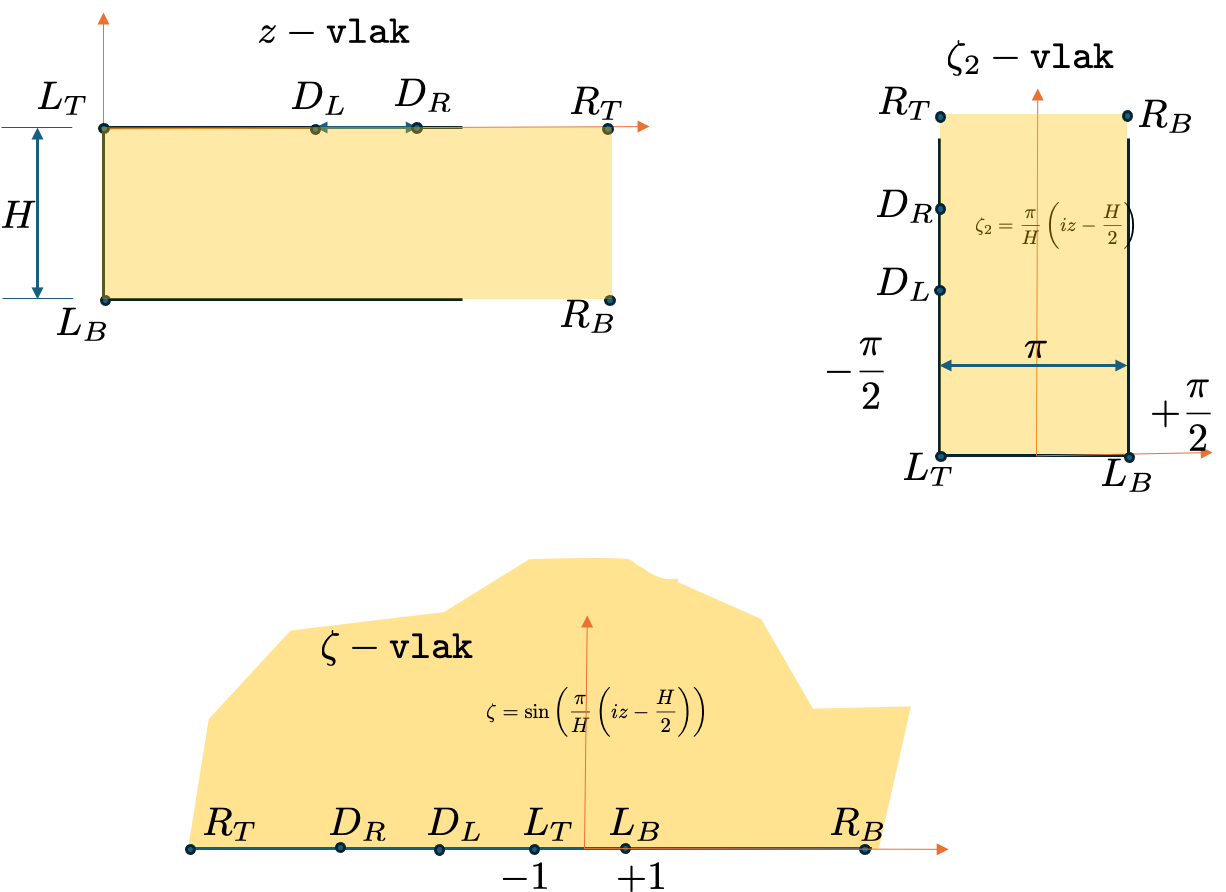
\includegraphics[width=0.8\textwidth]{/Users/Theo/GRWMODELS/python/Stromingen/H2O051995/images/zeta_transforms_1-3}
\par\end{centering}
\caption{\label{fig:stappen1-3}De eerste 3 transformaties: Van de doorsnede,
het $z$-vlak naar de gekantelde en verschaalde doorsnede, het $\zeta_{1}$-vlak,
naar de platgeslagen doorsnede, het $\zeta$-vlak.}
\end{figure}

De doorsnede in het $z$-vlak wordt eerst linksom om 90 graden gekanteld
door vermenigvuldiging met $i$ en dan verschaald to het $\zeta_{2}$-vlak,
waarin punt $L_{t}$ dus $z=0$ overgaat in $\zeta_{2}=-\frac{\pi}{2}$
en punt $L_{b}$ d.w.z. punt $z=-iH$ overgaat in $\zeta_{2}=+\frac{\pi}{2}$.
Door hier de sinus transformatie op los te laten worden de lijnen
$L_{t}-R_{r}$ en $L_{b}-R_{b}$ uitgeklapt op de horizontale as in
het $\zeta$-vlak

\[
\zeta=\sin\left(\frac{\pi}{H}\left(iz-\frac{H}{2}\right)\right)
\]

De volgende stap is om $\zeta$ te schalen en te verschuiven naar
$\zeta_{3}$, waarbij linker en rechter oever van de sloot, $\zeta_{L}$
en $\zeta_{R}$ op $\zeta_{3}=-1$ en $\zeta_{3}=+1$ komen te liggen.
Dit kan met een lineaire transformatie

\begin{align*}
p\zeta_{D_{R}}+q & =-1\\
p\zeta_{D_{L}}+q & =+1
\end{align*}

Dit geeft

,

\begin{align*}
p & =\frac{2}{\zeta_{D_{L}}-\zeta_{D_{R}}}\\
q & =1-p\zeta_{D_{L}}
\end{align*}

zodat

\[
\zeta_{3}=p\zeta+q
\]

Het $\zeta_{3}$-vlak is weertgeven in fig. \ref{fig:stappen4-6}

\begin{figure}[h]
\centering
\begin{centering}
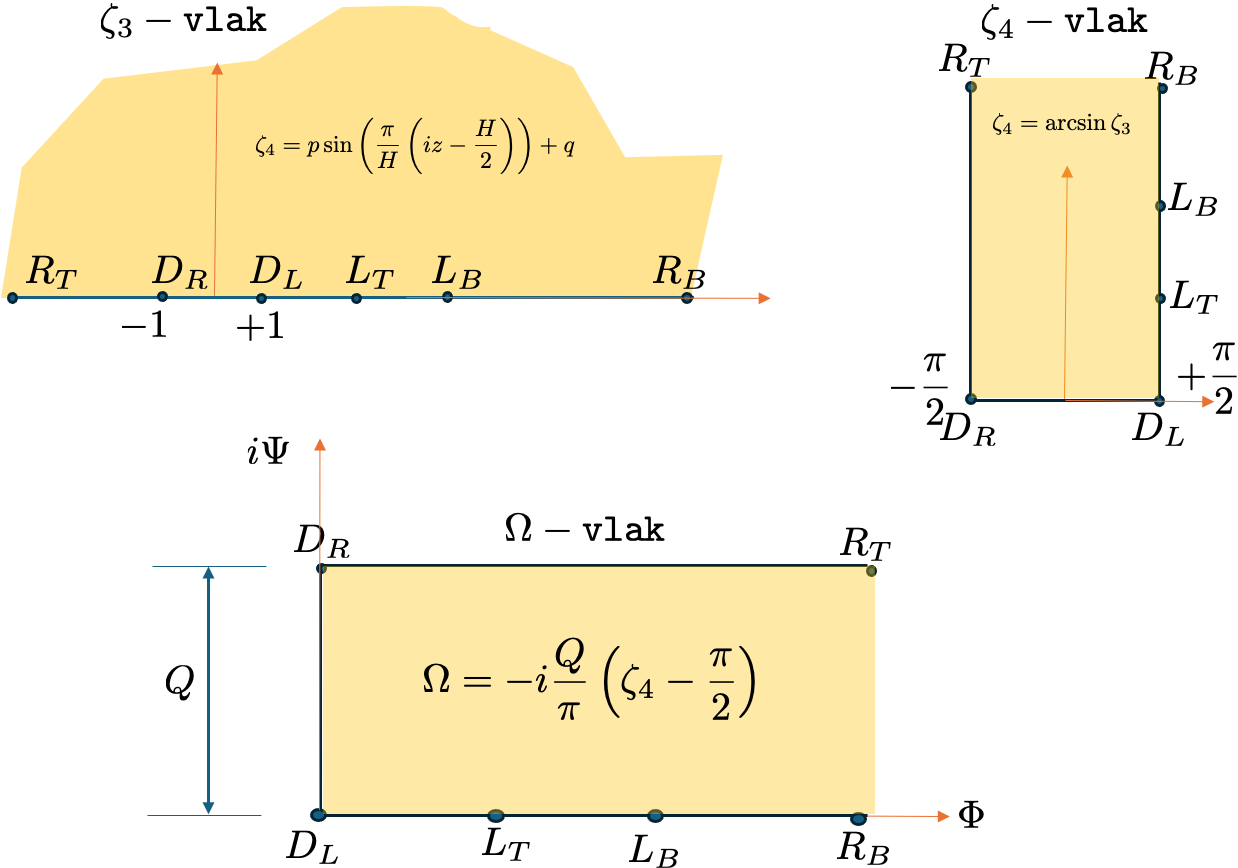
\includegraphics[width=0.8\textwidth]{/Users/Theo/GRWMODELS/python/Stromingen/H2O051995/images/zeta_transforms_4-6}
\par\end{centering}
\caption{\label{fig:stappen4-6}Visualisatie van de laatste 3 stappen, van
het $\zeta$-vlak in de voorgaande figuur naar het $\zeta_{3}$-vlak,
waarin de sloot op de coordinatgen $-1$ en $+1$ is gelegd, naar
het $\zeta_{4}$-vlak, waarin de rand $Rt-D_{R}$ en $D_{L}-R_{B}$
omhoog geklapt zijn, naar het uiteindelijke geroteerde en verschaalde
$\Omega$-vlak, waarin $D_{R}$ op $iQ$ en $D_{L}$ op 0 zijn gelegd.
Door de uitdrukking voor elk vlak in de laatste formule in te vullen
verkrijgt men de uiteindelijke conforme afbeelding van het oorspronkelijke
$z$-vlak (de doorsned) naar het $\Omega$-vlak, waarin de horizontale
lijne stroomlijnen zijn en de verticale potentiaallijnen.}

\end{figure}

Met de $\arcsin$-functie losgelaten op het $\zeta_{3}$-vlak worden
de horizontale as links van $D_{R}$ en rechts van $D_{L}$ omhoog
geklapt en krijgen deze twee punten respectievelijk de coördinaten
$-\frac{\pi}{2}$ en $+\frac{\pi}{2}$ in het $\zeta_{4}$-vlak.

\[
\zeta_{4}=\arcsin\left(\zeta_{3}\right)=\arcsin\left(p\zeta+q\right)
\]

Door de uiteindelijke verschaling van het$\zeta_{4}$-vlak naar het
$\Omega$-vlak moeten eerst de punten $\zeta_{4}=-\frac{\pi}{2}$
en $\zeta_{4}=\frac{\pi}{2}$ overgaan in respectievelijk $-Q$ en
0 waarna dit vlak door vermenigvuldiging met $-i$ nog een kwartslag
rechtsom wordt geroteerd tot het uiteindelijke $\Omega$-vlak 

\[
\Omega=-i\frac{Q}{\pi}\left(\zeta_{4}-\frac{\pi}{2}\right)
\]

Voegen we al deze stappen samen dan krijgen we de volgende transformatie
in een formule

\[
\Omega=-i\frac{Q}{\pi}\left(\arcsin\left(p\sin\left(\frac{\pi}{H}\left(iz-\frac{H}{2}\right)\right)+q\right)-\frac{\pi}{2}\right)
\]

Hierin zijn $p$ en $q$ berekend met de coördinaten van de hoekpunten
van de sloot in het $\zeta$-vlak zoals afgeleid.

De formule hiervoor is handig om de complexe potentiaal te berekenen
bij gegeven coordinaten in het vlak van de oorspronkelijkek doorsnede.
Het omgekeerde is ook mogelijk, namelijk om bij een gegeven complexe
potentiaal het bijbehorende punten in het $z$-vlak uit te rekenen.
Daarvoor keren we de zojuist afgeleide vergelijking binnenste buiten
en maken $z$ expliciet

\[
z=-iH\left(\frac{1}{2}+\frac{1}{\pi}\arcsin\left(\frac{\sin\left(i\frac{\pi}{Q}\Omega+\frac{\pi}{2}\right)-q}{p}\right)\right)
\]


\subsection{Slootweeerstand}

De slootweerstand is in feite de stijghoogte in de sloot minus die
op een referentiepunt waar geen stroming is. Het meest geschikte punt
lijkt $z=-0.5i$H, halverwege de hoogte van het watervoerende pakket
op $x=0$. Met $z=-0.5iH$ wordt $iz-\frac{H}{2}\rightarrow-0.5i^{2}H-0.5H=0$
zodat

\[
\Omega_{z=-0.5iH}=-i\frac{Q}{\pi}\left(\arcsin\left(q\right)-\frac{\pi}{2}\right)
\]

Met $p=0$ volgt uit de voorgaande lineaire transformatie $p\zeta+q$
dat

\begin{align*}
q & =-\frac{\zeta_{D_{L}}+\zeta_{D_{R}}}{\zeta_{D_{L}}-\zeta_{D_{R}}}
\end{align*}

Door $\zeta=\sin\left(\frac{\pi}{H}\left(iz-\frac{H}{2}\right)\right)$
in te vullen voor de linker en rechter oever van de infiltratiesloot,
resp. $x_{D_{L}}=a$ en $x_{D_{R}}=a+b$ vinden we

\begin{align*}
q & =-\frac{\sin\left(\frac{\pi}{H}\left(ia-\frac{H}{2}\right)\right)+\sin\left(\frac{\pi}{H}\left(i\left(a+b\right)-\frac{H}{2}\right)\right)}{\sin\left(\frac{\pi}{H}\left(ia-\frac{H}{2}\right)\right)-\sin\left(\frac{\pi}{H}\left(i\left(a+b\right)-\frac{H}{2}\right)\right)}
\end{align*}

\[
\sin\left(\xi\right)=\frac{\exp\left(+i\xi\right)-\exp\left(-i\xi\right)}{2i}
\]

\begin{align*}
\sin\left(\frac{\pi}{H}\left(ic-\frac{H}{2}\right)\right) & =\frac{\exp\left(+i\frac{\pi}{H}\left(ic-\frac{H}{2}\right)\right)-\exp\left(-i\frac{\pi}{H}\left(ic-\frac{H}{2}\right)\right)}{2i}\\
 & =\frac{\exp\left(-\pi\frac{c}{H}-i\frac{\pi}{2}\right)-\exp\left(+\pi\frac{c}{H}-i\frac{\pi}{2}\right)}{2i}\\
 & =\frac{\exp\left(-\pi\frac{c}{H}\right)\exp\left(-i\frac{\pi}{2}\right)-\exp\left(+\pi\frac{c}{H}\right)\exp\left(-i\frac{\pi}{2}\right)}{2i}\\
 & =\exp\left(-i\frac{\pi}{2}\right)\frac{\exp\left(-\pi\frac{c}{H}\right)-\exp\left(+\pi\frac{c}{H}\right)}{2i}
\end{align*}

met $\exp\left(-i\frac{\pi}{2}\right)=-i$ volgt

\begin{align*}
\sin\left(\frac{\pi}{H}\left(ic-\frac{H}{2}\right)\right) & =-\frac{\exp\left(-\pi\frac{c}{H}\right)-\exp\left(+\pi\frac{c}{H}\right)}{2}\\
 & =\sinh\left(-\pi\frac{c}{H}\right)
\end{align*}

voor $c=a+b$ volgt

\begin{align*}
q & =\frac{-\sinh\left(-\pi\frac{a}{H}\right)-\sinh\left(-\pi\frac{a+b}{H}\right)}{-\sinh\left(-\pi\frac{a}{H}\right)+\sinh\left(-\pi\frac{a+b}{H}\right)}\\
 & =\frac{\sinh\left(\pi\frac{a}{H}\right)+\sinh\left(\pi\frac{a+b}{H}\right)}{\sinh\left(\pi\frac{a}{H}\right)-\sinh\left(\pi\frac{a+b}{H}\right)}\\
 & =\frac{e^{\alpha}+e^{-\alpha}+e^{\alpha+\beta}-e^{-\alpha-\beta}}{e^{\alpha}+e^{-\alpha}-e^{\alpha+\beta}+e^{-\alpha-\beta}}\\
 & =\frac{e^{\alpha}+e^{-\alpha}+e^{\alpha}e^{\beta}-e^{-\alpha}e^{-\beta}}{e^{\alpha}+e^{-\alpha}-e^{\alpha}e^{\beta}+e^{-\alpha}e^{-\beta}}\\
 & =\frac{1+e^{-2\alpha}+e^{\beta}-e^{-2\alpha}e^{-\beta}}{1+e^{-2\alpha}-e^{\beta}+e^{-2\alpha}e^{-\beta}}
\end{align*}

Voor $a\rightarrow\infty$

\[
q=\frac{1+e^{\beta}}{1-e^{\beta}}=\frac{1+e^{\pi\frac{b}{H}}}{1-e^{\pi\frac{b}{H}}}
\]

Waaruit direct blijkt dat $q$ onafhankelijk is van de positie van
de sloot ($a$), mits $a\rightarrow\infty$. De waarde van de stijghoogte
op $z=-0.5iH$ kan nu direct worden berekend door $q$ in te vullen
in de vergelijking voor $\Omega_{z=-\infty}$.

\[
\Omega_{z=-0.5iH}=-i\frac{Q}{\pi}\left(\arcsin\left(\frac{1+\exp\left(\pi\frac{b}{H}\right)}{1-\exp\left(\pi\frac{b}{H}\right)}+0i\right)-\frac{\pi}{2}\right)
\]

De toevoering $0i$ zorgt ervoor dat Python het argument van de arcsin
als complex opvat en niet als reëel. Hiermee is de uitkomst van $\Omega_{z=-i\frac{H}{2}}$
gelijk aan de numeriek berekende $\Omega$ op het gekozen referentiepunt.
We hebben hiermee dus direct een waarde voor de slootweerstand verkregen.
De uitkomst is een reëel zoals ook moet voor een gewone stijghoogte.
In feite hebben we hiermee de gezochte stijghoogte van de sloot ten
opzichte van $z=-i\frac{H}{2}$ en is het vraagstuk volledig opgelost.

Verderop passen we in plaats van de intiële sinus transformatie de
exp transformatie toe, waarbij wel het punt op $x=-\infty$ kan worden
berekend omdat de aquifer dan van $-\infty$ naar $+\infty$ loopt.
Daar rekenen we de $\Omega_{z=-\infty}$ analytisch uit, die geijk
blijkt aan de hiervoor berekende uitkomst $\Omega_{z=-0.5iH}$. Ook
de numerieke waarden zijn gelijk aan deze analytische voor elke pakketdikte
$H$ en $b$ mits $a$ groot genoeg, terwijl bij de aanpak met intieel
de exp transformatie $a$ er (uiteraard) helemaal niet toe doet.

\subsection{Resultaten}

Fig. \ref{fig:De-doorsneden} geeft de berekende potentiaal en stroomfunctielijnen
in een zestal doorsneden. Elke doorsnede heeft dezelfde sloot van
10 m breedte gelegen op dezelfde afstand van de linker gesloten rand
van de doorsnede. De coördinaten van sloot staat steeds aangeven in
de koptekst van elke doorsnede. De doorsnedes verschillen alleen in
hun dikte, die loopt per doorsnede met 5 m op van 5 tot uiteindelijk
30 m. De totale infiltratie is in elke doorsnede hetzelfde, namelijk
Q=1 m$^{2}$/d. De antwoorden gelden dus voor een eenheidsinfiltratie.
Omdat de dikte verschillend zijn verschilt ook de schaal per doorsnede,
maar de ligging van de sloot ten opzichte van de linkerrand is steeds
hetzelfde. De potentiaal in de sloot is steeds nul. De blauwe dikke
stip links in de doorsnede, halverwege de hoogte is de plek waar de
potentiaal is berekend en de waarde is ernaast geplot.

Zoals Kees maas al aantoonde, zien we dat de potentiaal oploopt met
de hoogte van de doorsnede. Zijn argument dat ,,Dik freatisch pakket
infiltreert niet lekker'' blijkt dan ook hier uit deze resultaten.

\begin{figure}[h]
\centering
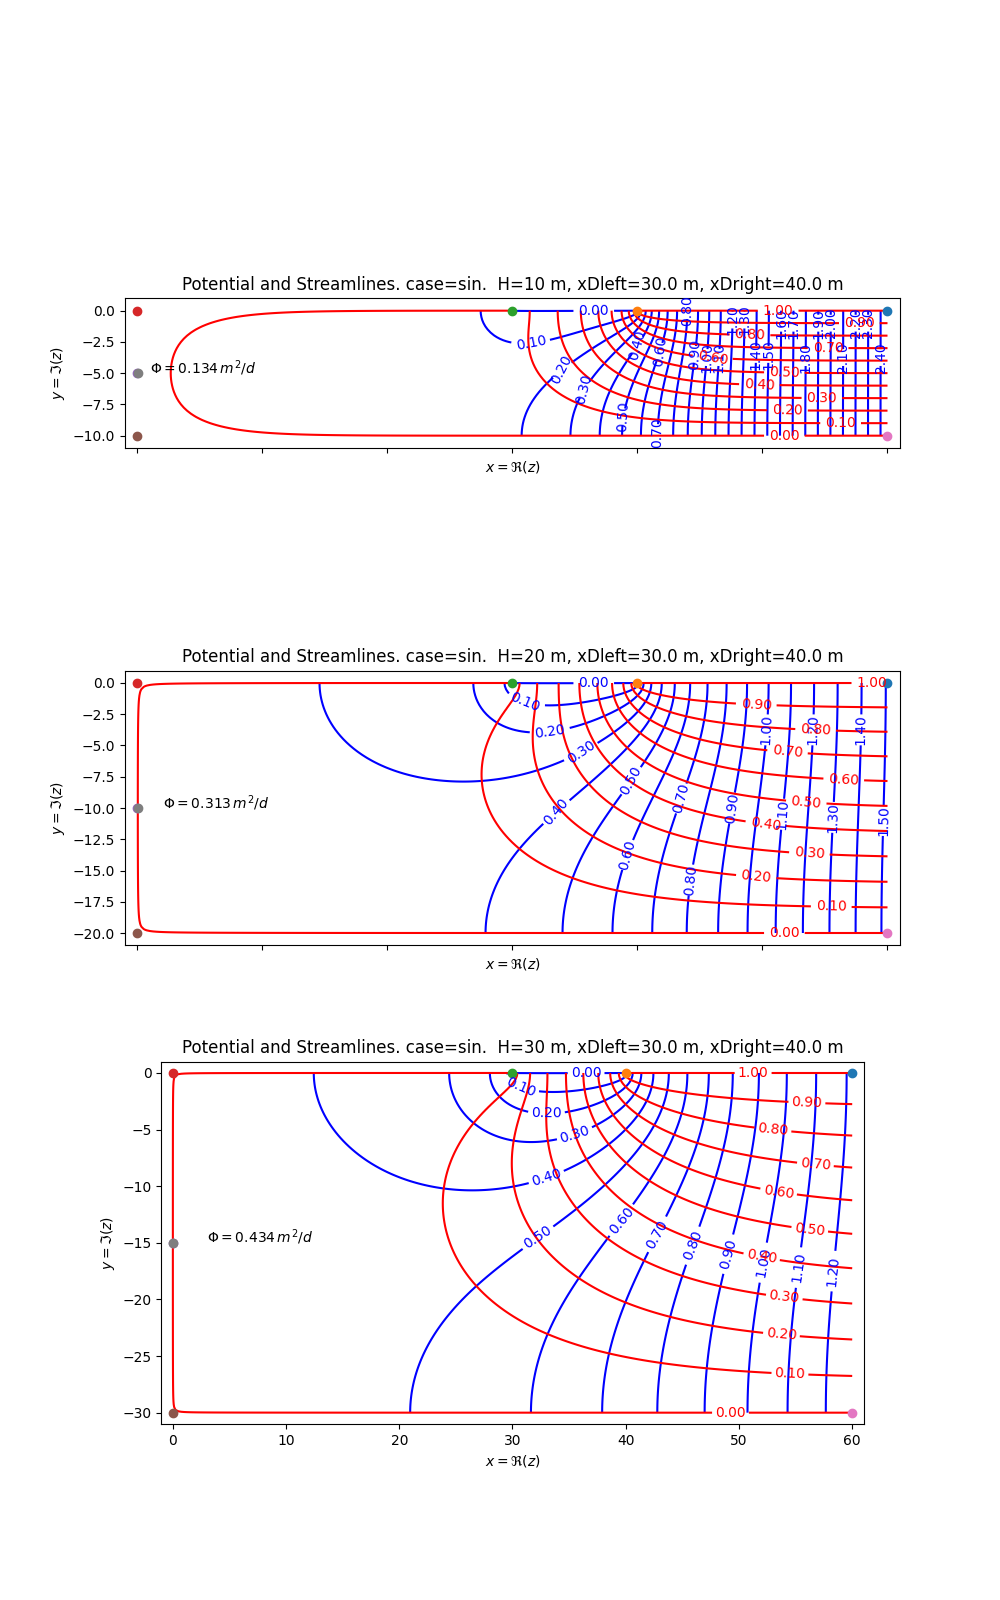
\includegraphics[width=0.8\textwidth]{/Users/Theo/GRWMODELS/python/Stromingen/H2O051995/images/sections_sin}

\caption{\label{fig:De-doorsneden}De doorsneden voor toenemende pakkedikte,
vaste slootbreedte en vaste totale infiltratie. Het getal in elke
figuur geeft de potentiaal op de plek van de blauwe punt, die in de
sloot is gelijk aan nul. De Buitenste stroomlijn is voor $\Psi=0.0001Q$
en $\Psi=0.9999Q$ zodat de lijn net binnen de doorsnede valt.}

\end{figure}

De vraag is nu wel of hier alles mee is gezegd. Immers een dikker
pakket bij dezelfde doorlatendheid en hetzelfde infitratiedebiet heeft
een kleiner verhang stroomafwaarts. Er is dus altijd een afstand waarop
het dikke pakket het wel gaat winnen van de extra weerstand die het
nabij de sloot opwekt. We kunnen dit met onze analytische oplossing
gemakkelijk controleren door de potentiaal langs de top en de basis
van het watervoerend pakket te berekenen. Het resultaat staat in fig.
\ref{fig:Potentiaal-langs-de-top-en-basis}. De linkerrand van de
doorsnede ligt op $x=\Re(z)=0$. De sloot ligt tussen $30\le x\le40$
en heeft altijd potentiaal 0. De hoogte van de doorsnede staat in
de legenda. De getrokken lijn van elke kleur is de potentiaal aan
de bovenzijde van de doorsnede; de lijn met de stippen die aan de
basis van de doorsnede. De potentiaal is links van de sloot lager
dan in de sloot en wordt constant in de richting van de rand, waar
geen stroming meer is. De slootweerstand is geijk aan het verschil
tussen de potentiaal in de sloot (0) en die nabij $x=0$. Rechts van
de sloot daalt de potentiaal als gevolg van de stroom $Q$. Hier zien
we duidelijk dat de daling sterker is wanneer de vaste stroom $Q$
door een dunner pakket wordt afgevoerd. Het is direct duidelijk dat
een dun pakket rechts van de sloot beduidend meer weerstand laat zien
dan een dik pakket. Al op beperkte afstand van de sloot overstijgt
het potentiaalverlies door de afstroming naar rechts die als gevolg
van de intrede via de sloot. Hoe dunner het pakket hoe lager dit intredeverlies
en hoe groter het afstroomverlies. Verdict, een dun pakket infiltreert
bij nader inzien toch niet zo heel lekker, ook al is het intrede verlies
daarvan kleiner dan van een dik pakket bij hetzerlfde debiet en dezelfde
doorlatendheid. Bij stroming over enige afstand, zoals bij kuntmatige
infiltratie het geval is, is het verlies van potentiaal door de geringe
dikte van een dun pakket groter dan de winst van een geringere intredeweerstand
van het dunnere pakket.
\begin{center}
\begin{figure}[h]
\centering
\begin{centering}
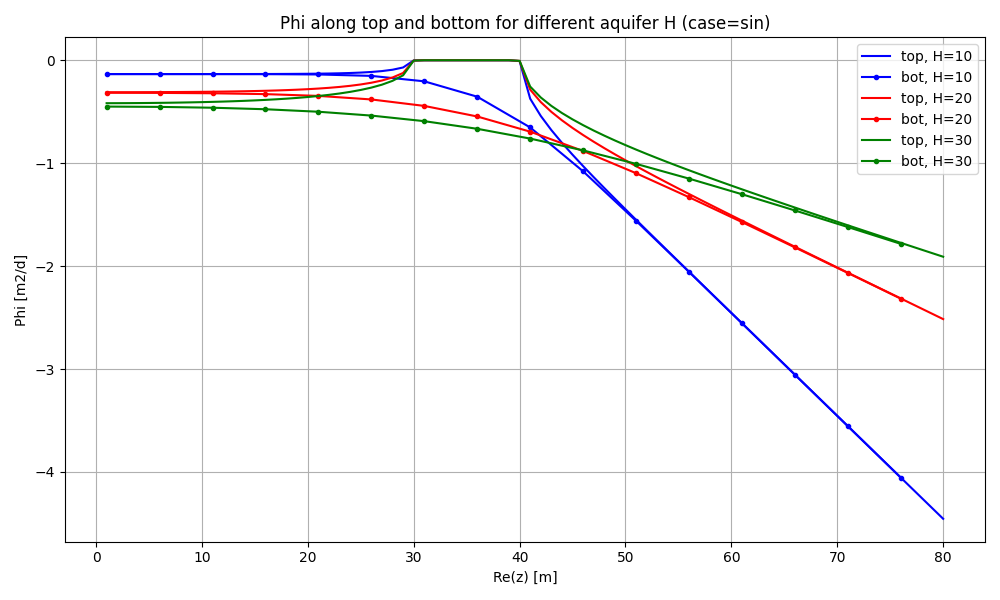
\includegraphics[width=0.8\textwidth]{/Users/Theo/GRWMODELS/python/Stromingen/H2O051995/images/tob_bot_potential_sin}
\par\end{centering}
\caption{\label{fig:Potentiaal-langs-de-top-en-basis}Potentiaal langs de top
en basis van de aquifer}

\end{figure}
\par\end{center}

\subsection{Via de exp-transformatie}

In plaats van de sinus-transformatie richting het $\zeta$-vlak kan
wellicht iets elegante de exp-transformatie worden gebruikt. Hierbij
loopt de doorsnede van $-\infty<x<+\infty$ en wordt het punt $z=-\infty$
afgebeeld op $\zeta=0$. Echter moet eerst de doorsnede lineair worden
verschaald zodat $z=0$ naar $i\pi$ en $z=-H$ naar 0 wordt verschaald.
Rotatie is nu niet nodig. We krijgen nu (zie fig. \ref{fig:van-z-naar-zeta-via-exp}):

\[
\zeta=\exp\left(\frac{\pi}{H}\left(z+iH\right)\right)
\]

\begin{figure}[h]
\centering
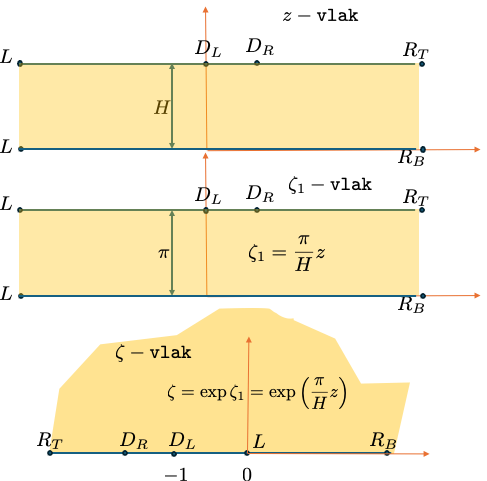
\includegraphics{../images/zeta_transforms_1-3_exp}

\caption{\label{fig:van-z-naar-zeta-via-exp}De transformatie van het $z$-vlak
naar het $\zeta$-vlak via de $exp$ transformatie.}

\end{figure}

De punten $L_{t}$ en $L_{b}$ worden beide op $\zeta=0$ afgbeeld
en de van de infiltratiesloot $D_{R}>z>D_{L}$ komen links daarvan
te liggen. Vanaf dit punt verloopt de verdere transformatie exact
hetzelfde als hiervoor. Eerst passen we een lineare tranformatie $\zeta_{4}=p\zeta+q$
toe die het $\zeta$-vlak zodanig verschaalt dat punt $\zeta_{D_{R}}\rightarrow-1$
en $\zeta_{D_{L}}\rightarrow+1$ in het $\zeta_{4}$-vlak, gevolgd
door het opklappen van de horizontale as links van $D_{R}$ en rechts
van $D_{L}$ en een laatste verschaling die ervoor zorgt dat punt
$D_{L}$ op $iQ$ en $D_{R}$ op $0$ komt te liggen

\[
\Omega=-i\frac{Q}{\pi}\left(\arcsin\left(p\zeta+q\right)-\frac{\pi}{2}\right)
\]

De totale transformatie kan nu in een formule worden opgeschreven

\[
\Omega=-i\frac{Q}{\pi}\left(\arcsin\left(p\exp\left(\frac{\pi}{H}\left(z+iH\right)\right)+q\right)-\frac{\pi}{2}\right)
\]

en omgekeerd

\[
z=-iH+\frac{H}{\pi}\ln\left(\frac{\sin\left(i\frac{\pi}{Q}\Omega+\frac{\pi}{2}\right)-q}{p}\right)
\]


\subsection{Resultaten}

Fig. \ref{fig:De-doorsneden-1} geeft de berekende potentiaal en stroomfunctielijnen
in een drietal doorsneden. Deze doorsneden zijn gelijk aan die hiervoor
behalve dat niet stopt op $x=0$ maar doorloopt naar $x=-\infty$.
De totale infiltratie Q is net als hiervoor gelijk aan $1$ m$^{2}$/d.
De potentiaal in de sloot is steeds nul. De blauwe dikke stip links
in de doorsnede, halverwege de hoogte is de plek waar de potentiaal
is berekend en de waarde is ernaast geplot. Deze blijken in 3 cijfers
nauwkeurig gelijk aan die in de voorgaande situatie. De waarden op
$x=\infty$ zijn nauwelijks anders. Ook hier zijn de uiterste stroomlijnen
$\Psi=0.0001Q$ en $\Psi=0.9999Q$ getekend. In de dunne doorsnede
blijft deze lijn binnen de getekende figuur, het als hiervoor, maar
voor de dikkere lopen deze stroomlijnen links buiten de figuur door
omdat de doorsnede nu daadwerkelijk doorloopt tot $x=-\infty$ in
plaats van slechts tot $x=0$. De lokatie van de sloot kan uiteraard
vrijelijk worden gekozen en zal altijd hetzelfde lijnenspel opleveren.
Hiervoor, waar de doorsnede op $x=0$ eindigt moet de sloot minimaal
op enkele keren de pakketdikte van de $x=0$ worden gelegd om te zorgen
dat de dichte rand op $x=0$ het stroombeeld niet beïnvloed. Uit de
gelijke potentiaalwaarden voor het referentiepunt is 30 m blijkbaar
voldoen.

\begin{figure}[h]
\centering
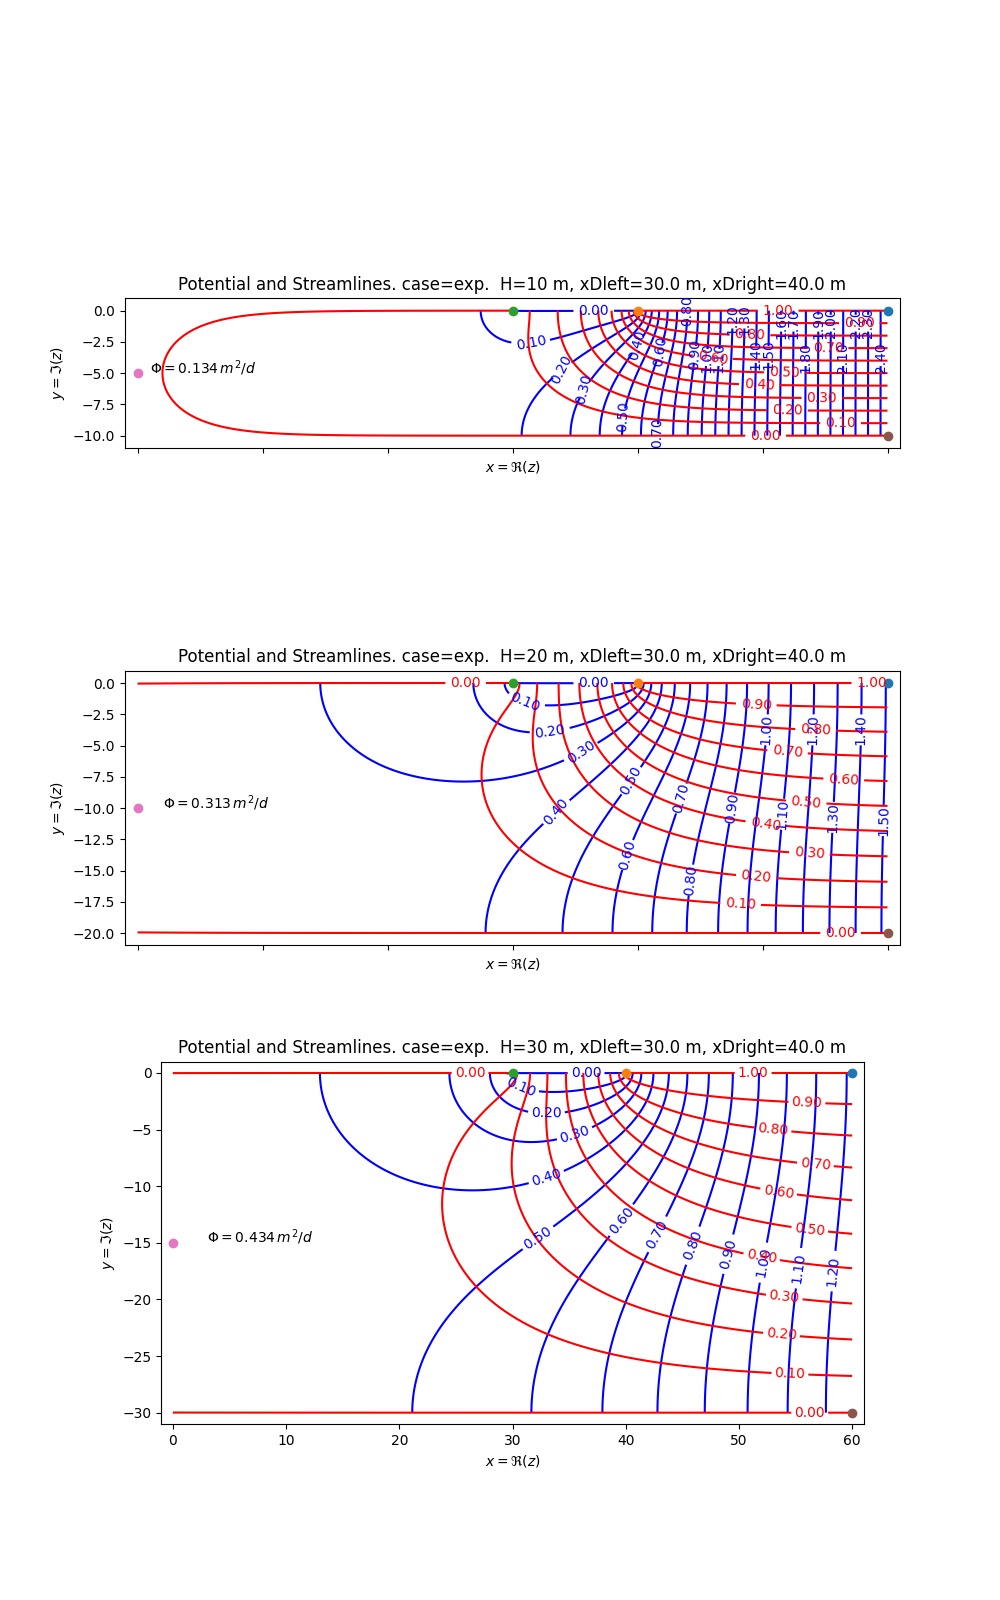
\includegraphics[width=0.8\textwidth]{/Users/Theo/GRWMODELS/python/Stromingen/H2O051995/images/sections_exp}

\caption{\label{fig:De-doorsneden-1}De doorsneden voor toenemende pakkedikte,
vaste slootbreedte en vaste totale infiltratie. Het getal in elke
figuur geeft de potentiaal op de plek van de blauwe punt, die in de
sloot is gelijk aan nul. De Buitenste stroomlijn is voor $\Psi=0.0001Q$
en $\Psi=0.9999Q$ zodat de lijn net binnen de doorsnede valt.}
\end{figure}

Evenals hiervoor kan de Potentiaal langs de top en de basis van de
drie doorsnedes worden berekend en getekend zoals gedaan in fig. \ref{fig:Potentiaal-langs-de-top-en-basis-1}
De uitkomsten zijn hetzelfde als hiervoor. De intredeweerstand neemt
toe met de dikte van het pakket maar de stromingweerstand is uiteraard
groter voor het dunnere pakket zoals direct blijkt uit het verloop
van de lijnen rechts van de sloot.
\begin{center}
\begin{figure}[h]
\centering
\begin{centering}
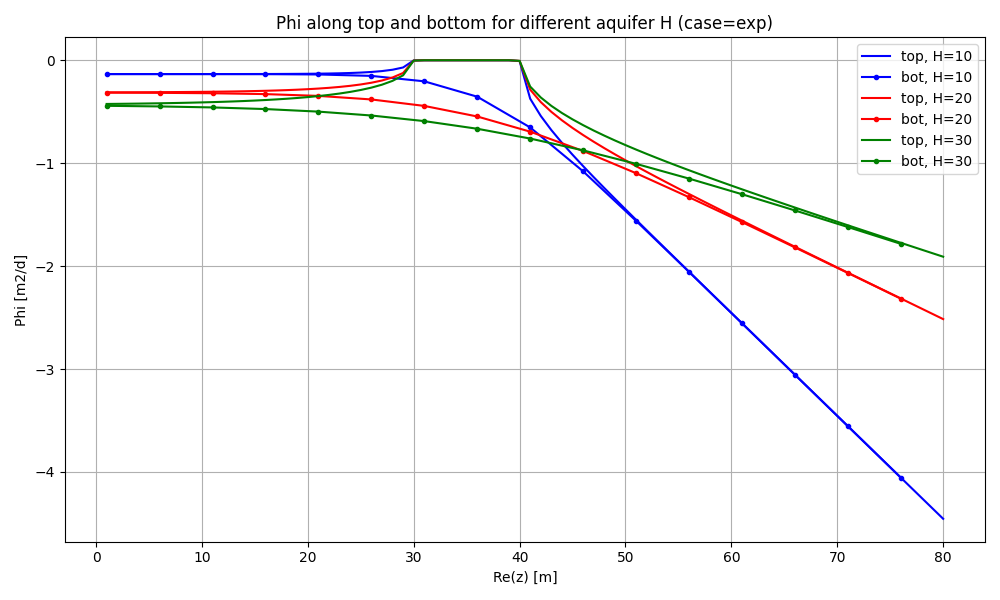
\includegraphics[width=0.8\textwidth]{/Users/Theo/GRWMODELS/python/Stromingen/H2O051995/images/tob_bot_potential_exp}
\par\end{centering}
\caption{\label{fig:Potentiaal-langs-de-top-en-basis-1}Potentiaal langs de
top en basis van de aquifer}
\end{figure}
\par\end{center}

\subsection{De potentiaal op $x=-\infty$}

De potentiaal op $x=-\infty$ bepaallt de waterstand in de sloot.
Wij hebben de transformatie zo gemaakt dat de potentiaal in de sloot
gelijk is aan 0. We kunnen om het slootpeil ten opzichte van die op
$x=-\infty$ krijgen door de waarde die de formule berekent op $x=\infty$
van $\Omega$ af te trekken.

Voor $x=\infty$ geldt dat de $\exp$ gelijk is aan nul

\[
\Omega_{z=-\infty}=-i\frac{Q}{\pi}\left(\arcsin\left(q\right)-\frac{\pi}{2}\right)
\]

Hiervoor hebben we $q$ reeds afgeleid, ingevuld leidt dit tot

\begin{align*}
q & =-\frac{\zeta_{D_{L}}+\zeta_{D_{R}}}{\zeta_{D_{L}}-\zeta_{D_{R}}}
\end{align*}

Door $\zeta=\exp\left(\frac{\pi}{H}\left(z+iH\right)\right)$ in te
vullen voor de linker en rechter oever van de infiltratiesloot, resp.
$x_{D_{L}}=a$ en $x_{D_{R}}=a+b$ vinden we

\begin{align*}
q & =-\frac{\exp\left(\frac{\pi}{H}\left(a+iH\right)\right)+\exp\left(\frac{\pi}{H}\left(a+b+iH\right)\right)}{\exp\left(\frac{\pi}{H}\left(a+iH\right)\right)-\exp\left(\frac{\pi}{H}\left(a+b+iH\right)\right)}\\
 & =-\frac{\exp\left(i\pi\right)+\exp\left(i\pi\right)\exp\left(\frac{\pi}{H}b\right)}{\exp\left(i\pi\right)-\exp\left(i\pi\right)\exp\left(\frac{\pi}{H}b\right)}\\
 & =-\frac{1+\exp\left(\frac{\pi}{H}b\right)}{1-\exp\left(\frac{\pi}{H}b\right)}
\end{align*}

Waaruit direct blijkt dat $q$ onafhankelijk is van de positie van
de sloot ($a$). De waarde van de stijghoogte op $x=-\infty$ kan
nu direct worden berekend door $q$ in te vullen in de vergelijking
voor $\Omega_{z=-\infty}$.

\[
\Omega_{z=-\infty}=-i\frac{Q}{\pi}\left(\arcsin\left(-\frac{1+\exp\left(\frac{\pi}{H}b\right)}{1-\exp\left(\frac{\pi}{H}b\right)}+0i\right)-\frac{\pi}{2}\right)
\]

De toevoering $0i$ zorgt ervoor dat Python het argument van de arcsin
als complex opvat en niet als reëel. Hiermee is de uitkomst van $\Omega_{z=-\infty}$
gelijk aan de numeriek berekende $\Omega$ op het gekozen referentiepunt.
We hebben hiermee dus direct een waarde voor de slootweerstand verkregen.
De uitkomst is een reëel zoals ook moet voor een gewone stijghoogte.
In feite hebben we hiermee de gezochte stijghoogte van de sloot ten
opzichte van $x=-\infty$ en is het vraagstuk volledig opgelost.

\section{Conclusie}

Overeenkomstig de afleiding van \cite{Ma95a} en de hier afgeleide
conforme afbeeldingen neemt de intredeweerstand van een infiltratiesloot
toe met de dikte van het watervoerende pakket, ook al blijven de doorlatendheid
en het het totale infiltraitedebiet daarbij behouden. Echter, het
dunnere pakket heeft bij gelijk debiet een groter potentiaalverhang
over het horizontale afstroomtraject. Er is hierdoor altijd een afstand
vanaf de infiltratiesloot waarop het dikkere pakket een kleinere totale
weerstand heeft dan het dunnere pakket. En als deze afstand kleiner
is dan de afstand tot de winmiddelen is de infiltraitiecapaciteit,
gerekend tussen sloot en winmiddelen, van het dikkere pakket toch
groter dan van het dunnere pakket. In zulke situaties infiltreert
een dik pakket misschien toch net wat lekkerder dan een dun pakket
(zie fig. \ref{fig:Potentiaal-langs-de-top-en-basis}).

\section{Opmerking}

Ik had er genoegen in dit al 30 jaar oude probleem nog eens op te
pakken en nader te bestuderen, en nog eens wat te doen met complexe
transformaties (conforme afbeeldingen). Het vraagstuk van de infiltratiesloot
met water dat naar een zijde afstroomt kan op meerdere manieren, afbeeldingen,
worden aangepakt. Ik vond persoonlijk altijd de algemeen toepasbare
Schwarz-Christoffel transformatie elegant maar lastig wegens de integraal
in de formule en de noodzaak om de plek van de punten $x_{i}$ op
de horizontale as te bepalen. Voor eenvoudige vraagstukken, zoals
het voorliggende, is dat redelijk tot goed te doen, daar geeft ook
Verruijt een voorbeeld van, maar in het algemeen blijft het lastig.
De andere aanpak is via het aaneenrijgen van een aantal basis-transformaties,
waarvan de exponent en de sinus (resp. log en de arscin) standaard
voorbeelden zijn. Ik heb de transformatie hier afgeleid via initieel
de sinus transformatie, waarvoor geldt dat de aquifer loopt van $0\le x\le\infty$.
Dat kan prima, maar dan moet de linker coördinaat van de sloot, $a$
voldoende groot zijn zodat het linker einde van de aquifer op $x=0$
er voor de potentiaal en stroomfunctie niet toe doen. Wat eleganter
kan het probleem ook worden opgelost door initieel de exponent transformatie
te gebruiken. Daarbij loopt de aquifer van $x=-\infty$ tot $x=+\infty$
en doet de linker coördinaat, $a$, van de sloot er helemaal niet
toe. Het resultaat is dan ook mathematisch exact gelijk aan de transformatie
met de Schwarz-Christoffel transformatie die Kees Maas toepaste. Kees
brengt de Potentiaal op $x=-\infty$ exact op 0, waardoor de potentiaal
van de slootbodem boven nul uitstijgt. Dat is echter triviaal. De
oplossing kent maar een gegeven potentiaal, die je op $x=-\infty$
of op de slootbodem kan opleggen of op welke plek dan ook. Door er
een constante bij op te tellen kunnen wel altijd de potentiaal op
$x=-\infty$ of op de slootbodem alsnog op nul zetten. De uitkomst
van de transformatie met de sinus is op het referentiepunt voldoende
ver links van de sloot in biede gevallen gelijk, omdat dat punt in
een gebied ligt waar de grondwaterdischarge willekeurig dicht bij
nul is.

Het was tamelijk rechttoe-rechtaan om in de transformatie met de exponent
voor de potentiaal op $x=-\infty$ een expliciete uitdrukking te vinden.
Ik wilde dat vervolgens ook proberen voor de aanpak met de intiële
sinus-transformatie. Dat bleek met enig doorzetten ook niet heel ingewikkeld
en was blij toen die gelijk bleek aan die met de intiële exponent-tranformatie,
wat natuurlijk ook zo moetst zijn.

Een persoonlijke anekdote is nog deze. Ik deed, meen ik, in 1973 mondeling
examen grondwatermechanica bij toen nog lector Arnold Verruijt. Ik
werd als studentje op zijn kamer ontvangen, waar hij zat met een voor
mij onbekende jonge man, die Otto Strack bleek te zijn. Zij hebben
me daar flink aan de tand gevoeld. En hadden uiteindelijk nog een
vraag. Die ging ook over de aquifer met het punt op $x=-\infty$ en
hoe ik dat zou aanpakken. Ik was niet helemaal goed op de hoogte van
de details van de exp-transformatie, en heb toen gezegd hoe ik in
dat geval de sinus-transformatie zou toepassen en dan het punt $x=0$
gewoon ver genoeg links van mijn probleem zo leggen zodat die rand
er voor de uitkomst niet toe deed. Dat vonden ze beiden goed, en ik
kreen een tien. En nu, na 52 jaar heb ik dan toch de exponent-transformatie
een keer zelf toegepast.
\begin{thebibliography}{Ollsthoorn (1995)}
\bibitem[Maas (1995a)]{Ma95a}Maas, K. (1995) DIk pakket infiltreert
niet lekker. H2O 28, No. 5, 152-153.

\bibitem[Maas (1995b)]{Ma95b}Maas, K. (1995) Nawoord van de auteur:
Dun blijft de mode ... H2O, Vol 28, No. 7, p203

\bibitem[Ollsthoorn (1995)]{O95}Olsthoorn, T.N. (1995) Hoe dikker
hoe better. H2O, Vol. 28, No. 7, p202-203.

\bibitem[Bot (1995)]{B95}Bot, A.P. (1995) Hoe dikker hoe beter. H2O,
Vol 28, No. 7, p203

\bibitem[Verruijt (1970)]{Verr70}Verruijt, A (1970) Theory of Groundwater
Flow. MacMillan, Pitman Presss, Bath GBr.

\end{thebibliography}


\end{document}
